\documentclass[12pt]{article} 
\usepackage{amsmath}
\usepackage{cancel}
\usepackage{algorithm}
\usepackage{graphicx}
\usepackage[noend]{algpseudocode}

\begin{document}

\begin{titlepage}

    \title{
        Method of Manufactured Solution Applied to SWIRL's Speed of Sound Integration
    Technique}


    \author{ Jeffrey Severino \\
        University of Toledo \\
        Toledo, OH  43606 \\
    email: jseveri@rockets.utoledo.edu}


    \maketitle

\end{titlepage}

\section{Introduction}
The Method of Manufactured Solutions (MMS) is a process for generating an 
analytical solution for a code that provides the numerical solution for a 
given domain. The goal of MMS is to establish a manufactured solution that can 
be used to establish the accuracy of the code within question. For this study, 
SWIRL, a code used to calculate the radial modes within an infinitely long duct
is being validated through code verification. SWIRL accepts a given mean flow and 
uses numerical integration to obtain the speed of sound. The integration technique
is found to be the composite trapezoidal rule through asymptotic error analysis.


\section{Methods}
The SWIRL code requires two mean flow parameters as a function of radius, $M_x$
, and $M_{\theta}$. The speed of sound, $\widetilde{A}$ is calculated by 
integrating $M_{\theta}$ with respect to r. To verify that SWIRL is handling 
and returning the accompanying mean flow parameters, the error between the 
mean flow input and output variables are computed. Since the trapezoidal rule
is used to numerically integrate $M_{\theta}$, the discretization error and 
order of accuracy is computed. Since finite differencing schemes are to be used 
on the result of this integration, it is crucial to accompany the integration 
with methods of equal or less order of accuracy. This will be determined by 
applying another MMS on the eigenproblem which will also have an order of 
accuracy.

\subsection{Theory}

If the flow contains a swirling component,
then the primitive variables are nonuniform through the flow, and mean flow assumptions are not valid. To account to this,
we integrate the momentum equation in the radial direction with
respect to the radius. 

Integrating the radial momentum equation yields,
%Equation (2.5) in Kousen's work is,

\[P = \int_{\tilde{r}}^{1} \frac{\bar{\rho} V_{\theta}^2}{\tilde{r}} d\tilde{r}\] 

where $\tilde{r}$ is the radius dimensional radius normalized 
by the tip diameter $r_t = r_{max}$

To show the work, we will start with the dimensional form of the equation and
differentiate both sides,
\[
    \frac{\bar{\rho} v_{\theta}^2}{r} 
    =\frac{\partial P}{\partial r}.
\]
Applying separation of variables,
\[
    \int_{r}^{r_{max}}
    \frac{\bar{\rho} v_{\theta}^2}{r} \partial r 
    =-\int_{P(r)}^{P(r_{max})}\partial p
\]

Since $\tilde{r} = r/r_{max}$,
\[r = \tilde{r}r_{max}.\]
Taking total derivatives (i.e. applying chain rule),
\[dr = d(\tilde{r}r_{max}) = d(\tilde{r})r_{max}\]
Substituting these back in and evaluating the right hand side,
\[
    \int_{\tilde{r}}^{1} \frac{\bar{\rho} v_{\theta}^2}{\tilde{r}}\partial \tilde{r} 
    =P(1)-P(\tilde{r})
\]

For reference the minimum value of $\tilde{r}$ is

\[\sigma = \frac{r_{max}}{r_{min}}\]

For the radial derivative, the definition of the speed of sound is utilized,
\[\frac{\partial A^2}{\partial r } =
\frac{\partial}{\partial r} \left( \frac{\gamma P}{\rho} \right).\]

Using the quotient rule, we can extract the definition of the speed of sound.

\begin{align*}
&= \frac{\partial P}{\partial r} \frac{\gamma \bar{\rho}}{\bar{\rho}^2} -
\left(
    \frac{\gamma P}{\bar{\rho}^2} 
\right) 
\frac{\partial \bar{\rho}}{\partial r}\\
&=  \frac{\partial P}{\partial r} \frac{\gamma }{\bar{\rho}} -
\left( \frac{A^2}{\bar{\rho}} \right) 
\frac{\partial \bar{\rho} }{\partial r}\\
\text{Using isentropic condition } \partial P/A^2 =
\partial \rho \rightarrow 
&= \frac{\partial P}{\partial r} \frac{\gamma }{\bar{\rho}} -
\left( \frac{1}{\bar{\rho}} \right) \frac{\partial  P }{\partial r}\\
\frac{\partial A^2}{\partial r} 
&= \frac{\partial P}{\partial r} \frac{\gamma - 1}{\bar{\rho}}  \\ \text{or..}
    \frac{\bar{\rho}}{\gamma -1}\frac{\partial A^2}{\partial r} &= \frac{\partial P}{\partial r} 
\end{align*}


Going back to the radial momentum equation, and rearranging the 

\begin{align*}
    \frac{\bar{\rho} v_{\theta}^2}{r} 
&=\frac{\partial P}{\partial r}\\
\frac{\cancel{
        \bar{\rho}
} v_{\theta}^2}{r} 
&=\frac{\cancel{\bar{\rho}}}{\gamma -1}\frac{\partial A^2}{\partial r}\\
    \frac{v_{\theta}^2}{r}\left(\gamma -1\right) &= \frac{\partial A^2}{\partial r}
\end{align*}
To start the nondimensionalization, we define,

\begin{align*}
    M_{\theta} &= \frac{V_{\theta}}{A} \\ 
    \widetilde{r} &= \frac{r}{r_{max}}  \\
    \widetilde{A} &= \frac{A}{A_{r,max}}  \\
    A &= \widetilde{A}{A_{r,max}} \\
    r &= \widetilde{r}{r_{max}}\\
    \frac{\partial}{\partial r} &=
    \frac{\partial \widetilde{r}}{\partial r} \frac{\partial}{\partial \widetilde{r}}\\
                                &= \frac{1}{r_{max}}\frac{\partial}{\partial \widetilde{r}}
\end{align*}
Dividing by $A$,
\begin{align*}
    \frac{M_{\theta}^2}{r}\left(\gamma - 1\right) 
&= \frac{\partial A^2}{\partial r} \frac{1}{A^2}
\end{align*}

%At this point we can either find the derivative of  $\bar{A}$ or the integral of
%$M_{\theta}$ with respect to r
%\begin{enumerate}
%    \item
%\begin{align*}
%\text{Integrating both sides } \int_{r}^{r_{max}}\frac{M_{\theta}}{r}\left(\gamma - 1\right){\partial r}  &=\int_{A^2(r)}^{A^2(r_{max})}\frac{1}{A^2}  {\partial A^2}\\
%\int_{r}^{r_{max}}\frac{M^2_{\theta}}{r}\left(\gamma - 1\right){\partial r}  &=ln(A^2(r_{max})) - ln(A^2(r)) \\
%\int_{r}^{r_{max}}\frac{M^2_{\theta}}{r}\left(\gamma - 1\right){\partial r}  &=ln\left(\frac{A^2(r_{max})}{A^2(r)}\right) 
%\end{align*}
%
%Defining non dimensional speed of sound $\tilde{A} = \frac{A(r)}{A(r_{max})}$
%\begin{align*}
%\int_{r}^{r_{max}}\frac{M_{\theta}}{r}\left(\gamma - 1\right){\partial r}  &=ln\left(\frac{1}{\tilde{A}^2}\right) \\
%&= -2ln(\tilde{A})\\
%\tilde{A}(r) &= exp\left[-\int_{r}^{r_{max}}\frac{M_{\theta}}{r}\frac{\left(\gamma - 1\right)}{2}{\partial r}\right] \\ \text{replacing r with }\tilde{r} \rightarrow \tilde{A}(r) &= exp\left[-\int_{r}^{r_{max}}\frac{M_{\theta}}{r}\frac{\left(\gamma - 1\right)}{2}{\partial r}\right]		\\
%\tilde{A}(\tilde{r}) &= exp\left[\left(\frac{1 - \gamma}{2}\right)\int_{\tilde{r}}^{1}\frac{M_{\theta}}{\tilde{r}}{\partial \tilde{r}}\right]	
%\end{align*}
%\item Or we can differentiate
%\end{enumerate}
%Solving for $M_{\theta}$ ,
%\begin{align*}
%M_{\theta}^2 
%&= \frac{\partial A^2}{\partial r} \frac{r}{A^2 \left(\gamma - 1\right)}
%\end{align*}
Nondimensionalizing:

Plugging in,

\begin{align} 
    M_{\theta}^2
    \frac{\left( \gamma - 1 \right)}{\widetilde{r} r_{max}} &=
    \frac{1}{(\widetilde{A}A_{r,max})^2}\frac{A_{r,max}^2}{r_{max}}
    \frac{\partial \widetilde{A}^2}{\partial \widetilde{r}} \nonumber \\
    M_{\theta}^2     \frac{\left( \gamma - 1 \right)}{\widetilde{r} } &=
    \frac{1}{\widetilde{A}^2}
    \frac{\partial \widetilde{A}^2}{\partial \widetilde{r}} \nonumber \\
    M_{\theta} &= \sqrt{\frac{\widetilde{r}}{(\gamma-1) \widetilde{A}^2}
        \frac{\partial\widetilde{A}^2}{\partial \widetilde{r} }
    } \label{eq:Mthetabackcalculated}
\end{align}

3.1 Guidelines for Creating Manufactured Solutions states:
\begin{enumerate}
    \item  The manufactured solutions should be composed of smooth analytic 
        functions 
    \item The manufactured solutions should exercize every term in the governing
        equation that is being tested,
    \item The solution should have non trivial derivatives.  
    \item The solution derivatives should be bounded by a small constant. In this case
        this constant should prevent the function from becoming greater than 
        one.
    \item The solution should not prevent the code from running 
    \item The solution should be defined on a connected subset of two- or three-
        dimensional space to allow flexibility in chosing the domain of the PDE.
        Section 3.3.1 provides more information about this.
    \item The solution should coincide with the differential operators of the PDE.
        For example, the flux term in Fourier's law of conduction requires T to 
        be differentiable.
\end{enumerate}
With these guidelines, a function is specified for the speed of sound to conduct
a method of manufactured solutions on SWIRL's speed of sound numerical 
integration. This is checked by observing the tangential mach number 
produced from the speed of sound and comparing that to the tangential mach number
that has been analytically defined (See Equation \ref{eq:Mthetabackcalculated}).
\subsection{Procedure}

To test the integration code,  $M_{\theta}$ is defined as a result 
of differentiating the speed of sound. This is done opposed to integrating
$M_{\theta}$ as a preference, but a function can be defined for $M_{\theta}$, and 
then integrate to find what $\widetilde{A}$ should be. 
Instead, the procedure of choice is to back calculate what the appropriate 
$M_{\theta}$ is for a given expression for $\widetilde{A}$.

Since it is easier to take derivatives , we will solve for $M_{\theta}$ using 
Equation \ref{eq:Mthetabackcalculated} ,

\begin{align*}
    M_{\theta} = \sqrt{ \frac{\widetilde{r}}{(\gamma -1) \widetilde{A}^2} 
    \frac{\partial \widetilde{A}^2}{\partial \widetilde{r}}}
\end{align*}
This time we define the speed of sound with the subscript $Analytic$ to indicate 
that this is the analytical function of choice and has no physical relevance 
to the actual problem
\begin{align*}
    \widetilde{A}_{Analytic} = \cos \left( k \left( \widetilde{r} - \widetilde{r_{max}} \right) \right)
\end{align*}

Taking the derivative with respect to $\widetilde{r}$,

\begin{align*}
    \frac{\partial \widetilde{A}_{Analytic} }{\partial \widetilde{r}} &= 
    \frac{\partial }{\partial \widetilde{r}}\left( 
        \cos \left( k \left( \widetilde{r} - \widetilde{r_{max}} \right) \right)
    \right)\\
    \frac{\partial \widetilde{A}_{Analytic}}{\partial \widetilde{r}} &= 
    -k\,\sin\left(k\,\left(r-r_{\mathrm{max}}\right)\right)
\end{align*}
Now we substitute this into the expression for $M_{\theta}$ in Equation 
\ref{eq:Mthetabackcalculated},

\begin{align*}
    M_{\theta} = \sqrt{2}\,\sqrt{-\frac{k\,r\,\sin\left(k\,\left(r-r_{\mathrm{max}}\right)\right)}{(\gamma - 1)\,\cos\left(k\,\left(r-r_{\mathrm{max}}\right)\right)}}
\end{align*} 



\subsection{Calculation of Observed Order-of-Accuracy}

To begin the method of manufactured solutions, the discretization error,
$\epsilon$ is defined as a function of radial grid spacing, $\Delta r$

\[ \epsilon = \epsilon(\Delta r) \]
The discretization error in the solution should be proportional to 
$\left( \Delta r \right)^{\alpha}$ where $\alpha > 0$ is the theoretical order
for the computational method.  The error for each grid is expressed as 
\[ \epsilon_{M_{\theta}}(\Delta r) = |M_{\theta,Analytic}-M_{\theta,calc}|\]
where $M_{\theta,Analytic}$ is the tangential mach number that is defined from the
speed of sound we also defined and the $M_{\theta,calc}$ is the result from 
SWIRL. The $\Delta r$ is to indicate that this is a discretization error for a
specific grid spacing. Applying the same concept to to the speed of sound,

If we define this error on various grid sizes and compute $\epsilon$ for
each grid, the observed order of accuracy can be estimated and compared to
the theoretical order of accuracy. For instance, if the numerical soution
is second-order accurate and the error is converging to a value, the L2 norm of
the error will decrease by a factor of 4 for every halving of the grid cell 
size. 
Since the input variables should remain unchanged (except from minor changes 
from the Akima interpolation), the error for the axial and tangential mach 
number should be zero. As for the speed of sound, since we are using an analytic
expression for the tangential mach number, we know what the theoretical result
would be from the numerical integration technique as shown above. 
Similarly we define the discretization error for the speed of sound.

\[ \epsilon_{A}(\Delta r) = |A_{Analytic}-A_{calc}|\]

For a perfect answer, we expect $\epsilon$ to be zero. Since a Taylor series can 
be used to derive the numerical schemes, we know that the truncation of higher
order terms is what indicates the error we expect from using a scheme that 
is constructed with such truncated Taylor series.

%\text{H.O.T}
We expect the error at each grid point $j$ to satisfy the following,
\begin{align*}
    0 &= |A_{Analytic}(r_j) - A_{calc}(r_j)| \\
    \widetilde{A}_{Analytic}(r_j) &= \widetilde{A}_{calc}(r_j) +
    (\Delta r)^{\alpha} \beta(r_j)  + H.O.T
\end{align*}

where the value of $\beta(r_j)$ does not change with grid spacing, and 
$\alpha$ is the asymptotic order of accuracy of the method. It is important to
note that the numerical method recovers the original equations as the grid 
spacing approached zero.

Subtracting $A_{Analytic}$ from both sides gives

\begin{align*}
    A_{calc}(r_j) - A_{Analytic}(r_j) &= A_{Analytic}(r_j) - A_{Analytic}(r_j)
    + \beta(r_j) (\Delta r)^{\alpha} \\
    \epsilon_A(r_j)(\Delta r) &= \beta(r_j) (\Delta r)^{\alpha}
\end{align*}



To estimate the order of accuracy of the accuracy, we define the global errors 
by calculating the L2 Norm of the error which is denoted as $\hat{\epsilon}_A$ 

% \begin{align*}
%     0 &=|A_{Analytic}(r_j)-A_{calc}(r_j)| \\
%     A_{calc}(r_j) &= A_{Analytic}(r_j) + \beta(r_j) (\Delta r)^{\alpha} + 
% \end{align*}

\begin{align*}
    \hat{\epsilon}_A = \sqrt{\frac{1}{N}\sum_{j=1}^{N} \epsilon(r_j)^2  }
\end{align*}

\begin{align*}
    \hat{\beta}_A(r_j) = \sqrt{\frac{1}{N}\sum_{j=1}^{N} \beta(r_j)^2  }
\end{align*}
As the grid density increases, $\hat{\beta}$ should asymptote to a constant 
value. Given two grid densities, $\Delta r$ and $\sigma\Delta r$, and assuming
that the leading error term is much larger than any other error term,

\begin{align*}
    \hat{\epsilon}_{grid 1} &= \hat{\epsilon}(\Delta r) = \hat{\beta}(\Delta r)^{\alpha} \\
    \hat{\epsilon}_{grid 2} &= \hat{\epsilon}(\sigma \Delta r) = \hat{\beta}(\sigma \Delta r)^{\alpha} \\
                            &= \hat{\beta}(\Delta r)^{\alpha} \sigma^{\alpha}
\end{align*}

The ratio of two errors is given by,

\begin{align*}
    \frac{\hat{\epsilon}_{grid 2}}{\hat{\epsilon}_{grid 1}} &= 
    \frac{\hat{\beta}(\Delta r )^{\alpha}}{\hat{\beta}(\Delta r )^{\alpha}} \sigma^{\alpha} \\ &= \sigma^{\alpha}
\end{align*}

Thus, $\alpha$,the asymptotic rate of convergence is computed as follows 

\begin{align*}
    \alpha = \frac{
        \ln \frac{
            \hat{\epsilon}_{grid 2}
    }{\hat{\epsilon}_{grid 1} }}
    {\ln\left( \sigma \right) }
\end{align*}

Defining  for a doubling of grid points ,

\begin{align*}
    \alpha = \frac{\ln \left( \hat{\epsilon}\left( \frac{1}{2}\Delta  r\right)
            \right) -\ln \left( \hat{\epsilon}\left( \Delta  r\right)
    \right)}{\ln \left( \frac{1}{2} \right)}
\end{align*}



\section{Results}

To confirm that the mean flow was consistent throughout SWIRL's computation,
the input mean flow data was compared to the output mean flow data to ensure 
that the mean flow variables remain unchanged.
Then, by setting $k$ equal to $0.1$ and starting with 9 grid points and ending
at 33, we can compute the global errors along with the asymptotic rate of 
convergence.  

% % \begin{figure}[h!]
%     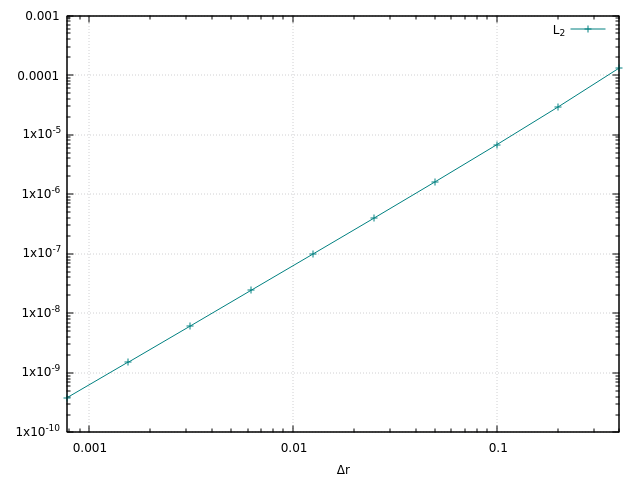
\includegraphics[width=\textwidth]{Figures/l2vDr}
% \end{figure}


% \begin{figure}[h]
%     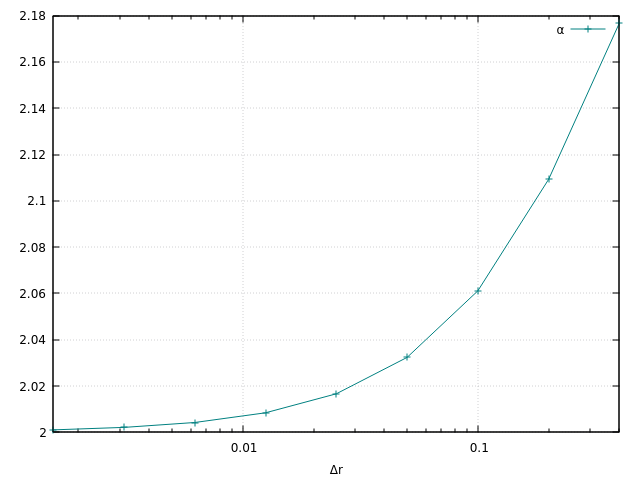
\includegraphics[width=\textwidth]{Figures/alphaVdr}
% \end{figure}


\section{Conclusion}
\section{Appendix}

\subsection{Error Analysis}


Reference: A. Ralston, A first course in numerical analysis 2nd edition

\subsubsection{Exact Polynomial Approximation}


Say we have some discrete data,

\begin{equation*}
    \left( x_{i},y_2 \right),\left( x_2, y_2 \right), \dots , \left( x_n,y_n \right)
\end{equation*}
We want to find a polynomial of the LEAST degree that gits these points exactly. 
Such a polynomial is called a Lagrange Polynomial. If in addition you supply a
function, or derivative value, you can use Hermitie intepolation to help the 
desired fitted polynomial handle sudden changes (?)

For Lagrange Polynomials, the general form is,

\begin{equation*}
    p\left( x_i  \right) =
    \sum_{j=1}^{n} l_j(x_i) f(x_j) + \underbrace{\frac{f^{(n)}\left( c \right)}
    {n!}p_n(x_i)}_{\text{Error at } x_i},
\end{equation*}
where,

\begin{equation*}
    p_n(x_i) = \prod_{j = 1}^{n} \left( x_i - x_j \right) 
\end{equation*}

\begin{equation*}
    p_n(x_i) =  \left( x_{i} - x_{j} \right) 
    \left( x_i - x_{i+1} \right)
    \left( x_i - x_{i+2} \right)
    \left( x_i - x_{i+3} \right) \dots
    ( x_i - x_n)
\end{equation*}

So if we have two data points $x_i$ and $x_{i+1}$, the function of least degree
that fits the data \textit{exactly} for a Langrange interpolation is,

\begin{equation*}
    p(x_i) = l_{i}(x_i)f(x_{i}) + l_{i+1}(x_{i+1})f(x_{i+1}) + \left[\text{
        Error at $x_i$}
    \right]
\end{equation*}

Note that I said \textit{exactly}! So I will drop the error term\dots

Then we \textit{claim} that

\begin{align*}
    p(x_i) =  
    l_i\left( x_i\right)f_i\left( x_i\right) + 
    l_{i+1}\left( x_{i+1}\right)f_{i+1}\left( x_{i+1}\right) 
\end{align*}

which means that we also claim that
\begin{align*}
    l_i(x) = \frac{x - x_{i+1}}{x_{i} - x_{i+1}} \\
    l_{i+1}(x) = \frac{x - x_{i}}{x_{i+1} - x_{i}}
\end{align*}

if $x = x_i$,
\[ l_i(x_i) = \frac{x_i - x_{i+1}}{x_i - x_{i+1} }= 1\], 
\[l_{i + 1}(x_i) = \frac{x_i-x_i}{x_{i+1} - x_{i}} = 0\]
and 
if $x = x_{i+1}$,

\[ l_i(x_{i+1}) = \frac{x_{i+1} - x_{i+1}}{x_i - x_{i+1} }= 0\], 
\[l_{i + 1}(x_{i+1}) = \frac{x_{i+1}-x_i}{x_{i+1} - x_{i}} = 1\]

let's see if $p\left( x \right)$ passes through these points exactly,

\begin{align*}
    p\left( x_i \right) &= 1 f_i(x_i) + 0 f\left( x_i  \right) =  f\left( x_i  \right) \\
    p\left( x_{i+1} \right) &= 1 f_{i+1}(x_{i+1}) + 0 f\left( x_{i+1}  \right) =  f\left( x_{i+1}  \right) 
\end{align*}

Defining,

\begin{align*}
    \Delta x^+ &= x_{i+1} - x_i \\
    \hat{x} &= x - x_i 
\end{align*}
Using this on the Lagrange polynomial for two points gives 

\begin{align*}
    \left( \frac{
            \left( x - x_{i+1} \right)
            }{
            \left( x_i - x_{i+1} \right)
        }
        f_i
        + \frac{
            \left( x - x_i  \right)
            }{
            \left(x_{i+1}- x_i \right)
        }
        f_{i+1}
    \right) \\
    \left( 
        \frac{
            \left( x - \left( x_{i+1} \right) \right)
            }{
            \left( x_i - x_{i+1}\right)
        } 
        f_i + 
        \frac{
            \left( x + \left( -x_i \right) \right)
            }{
            \left( \left( x_{i+1} \right) + \left( -x_i \right) \right)
        }
        f_{i+1}
    \right) \\
    \left(
        \frac{
            (x-\left( \Delta x^+ + x_i \right)) 
            }{
            x_i - (\Delta x^+ + x_i)
        }
        f_i
        +
        \frac{ 
            \left( x + \left( \hat{x} - x \right) \right)
            }{
            \left( \left( \Delta x^+ + x_i \right) + \left( -x_i \right) \right)
        }
        f_{i+1}
    \right)  \\
    \left(
        \frac{
            (\left(x-x_i  \right) -\Delta x^+)   
            }{ 
            - \Delta x^+ 
        }
        f_i
        +
        \frac{
            \left(   \hat{x}    \right)
            }{\left( \left(  \Delta x^+ + x_i \right)  + \left( -x_i \right) \right)
        } f_{i+1}
    \right) \\
    \frac{
        \hat{x} - \Delta x^+
        }{
        -\Delta x^+
    }
    f_i
    +
    \frac{
        \hat{x}
        }{
        \Delta x^+
    }
    f_{i+1}
\end{align*}

The Lagrange polynomial is

\begin{equation*}
    \widetilde{f}\left( \hat{x} \right) 
    =
    \left( 
        \frac{\hat{x}}{\Delta x^+}f_{i+1} +
        \frac{\Delta x^+ - \hat{x}}{\Delta x^+}f_i
    \right)
\end{equation*}

\subsection{Integration}

Recall that 

\[ \hat{x} = x - x_i\]
Now we prepare to integrate,

\begin{align*}
    \int_{x_1}^{x_2} \widetilde{f} dx &=
    \int_{x_1-x_i}^{x_2-x_i} \widetilde{f} \frac{\partial x}{\partial \hat{x}}d\hat{x}\\
                                      &=
                                      \int_{x_1-x_i}^{x_2 - x_i} \widetilde{f} d\hat{x}
\end{align*}

In the interior of the domain $i = 1, iMax - 1$, the function is integrated 
from $\hat{x} = 0$ to $\hat{x} = \Delta x^+$. In other words ,the integration 
covers the complete range of the polynomial. Note that we are only integrating
over a single interval.

\begin{align*}
    \int_0^{\Delta x^+} \widetilde{f} d\hat{x}&=
    \int_0^{\Delta x^+}
    \left( 
        \frac{\hat{x}}{\Delta x^+}f_{i+1} +
        \frac{\Delta x^+ - \hat{x}}{\Delta x^+}f_i
\right) \\ &= 
\frac{1}{\Delta x^+}f_{i+1}
\int_{0}^{\Delta x^+} 
\left(\hat{x}  \right) d\hat{x}
+
\frac{1}{\Delta x^+}
f_{i}
\left(
    \int_{0}^{\Delta x^+} 
    \left( \Delta x^+  \right) d\hat{x}
    -
    \int_{0}^{\Delta x^+} 
    \left( 
        \hat{x}
    \right) d\hat{x}
\right)\\
           &=\frac{1}{\Delta x^+}
           \left( 
               f_{i+1}\left[ 
                   \frac{\left( \Delta x^+ \right)^2}{
                   2} - 0
               \right]_0^{\Delta x^+}
               +
               f_i
               \left[ 
\frac{\left( \Delta x^+ \right)^2}{
                   2} - 0
               \right]_0^{\Delta x^+}
           \right) \\ &=
           \frac{\left( \Delta x^+ \right)^2}{2 \Delta x^+}
           \left[ f_{i+1} +f_i\right] \\
           &= 
           \frac{\Delta x^+}{2 }
           \left[ f_{i+1} +f_i\right] 
\end{align*}
Which is the trapezoidal rule!
\subsection{Taylor Series Error Analysis}

Here we try to determine the order of accuracy of the trapezoidal rule. 
The Taylor series for the integral $F$ and for the function $f$ are:

\begin{align*}
    f_{i+1} &= f_i +
    \Delta x \frac{\partial f}{\partial x}|_i +
    \frac{\Delta x^2}{2} \frac{\partial^2 f}{\partial x^2}|_i +
    \mathcal{O}\left( \Delta x^3 \right) \\
    f_i &= f_i
\end{align*}
Summing the two gives,

\begin{align*}
f_i + f_{i+1} = 2 f_i  + \Delta x \frac{\partial f}{\partial x } +
\mathcal{O}\left( \Delta x^2 \right) 
\end{align*}
Multiplying by $\Delta x /2  $

\begin{align*}
    \frac{\Delta x}{2 }(f_i + f_{i+1} )= 
    f_i {\Delta x} + \frac{\Delta x ^2}{2}\frac{\partial f}{\partial x } +
\mathcal{O}\left( \Delta x^3 \right) 
\end{align*}


\subsection{Composie Trapezoidal Rule}
To account for the entire domain, we express our trapezoidal rule as the sum 
of sub intervals for a uniform grid, to do so we redefine the grid spacing,

\[\Delta x^+   = \frac{\Delta \widetilde{ x}^+  }{n - 1}   \]

where $\widetilde{x}+$ is the length of the domain
and $n$ is the total number of grid points. 

\begin{align*}
    \int_{x_1}^{x_n} \widetilde{f} d \hat{x} &= 
    \frac{\Delta x^+}{2} \sum_{i=1}^{n}
    \left( 
        f_i + f_{i+1}
    \right) \\ 
    &=
    \frac{\Delta x^+}{2}  
    \left[ 
        \left( f_1 + f_2 \right) +
        \left( f_2 + f_3 \right)  +\dots +
        \left( f_{n-2} + f_{n-1} \right) + 
        \left( f_{n-1} + f_{n} \right)  
    \right] \\
    &=
    \frac{\Delta x^+}{2}  
    \left[ 
        \left( f_1 +
            2f_2  +
         2f_3+\dots +
         2f_{n-2} + 
         2f_{n-1}  + 
         f_{n} \right)  
    \right] \\
    &=
    \frac{\Delta x^+}{2}
    \left[ 
        f_1 + f_n + 
        2 \sum_{i=2}^{n-1}
        f_i
    \right] \\
    &=
    \frac{\Delta x^+}{2}
    \left[ 
        f_1 + f_n \right] 
        + 
        \Delta x^+ \sum_{i=2}^{n-1}
    f_i
\end{align*}

Noe we can use A taylor series expansion on the composite trapezoidal rule to
get an order of accuracy

the summation will be expanded Around $ i \Delta x$ in order to interpret the sum 
as a Riemann sum
\begin{align*}
    f_1  &= f_1\\
    i\Delta x \frac{\partial f }{\partial x } +
    \frac{(i\Delta x)^2}{2!} \frac{\partial^2 f }{\partial x^2 } +
    \frac{(i\Delta x)^3}{3!} \frac{\partial^3 f }{\partial x^3 } + \dots
\end{align*}

Let's further simplify the Taylor series at the last grid point,
\begin{align*} 
    f_n &= f_1 + 
    \Delta \widetilde{x}^+\frac{\partial f }{\partial x  } +
    \frac{(\Delta \widetilde{x}^+)^2}{2!}\frac{\partial^2 f }{\partial x^2  } +
    \frac{(\Delta \widetilde{x}^+)^3}{3!}\frac{\partial^3 f }{\partial x^3  } + \dots \\
        &= 
        f_1 +
        \left( n - 1 \right)\Delta x^+ 
        \frac{\partial f}{\partial x} +
        \frac{\left( n - 1 \right)^2}{2}\Delta x^+ 
        \frac{\partial^2 f}{\partial x^2} +
        \frac{\left( n - 1 \right)^3}{3}\Delta x^+ 
        \frac{\partial^3 f}{\partial x^3}
\end{align*}

Okay this is a bit tricky, lets distribute the summation on the Taylor series 
expanded around each grid point. Since this Taylor Series expanison involves 
the 1st grid point we re-adjust our summation to show this.

\begin{align*}
    \sum_{i = 2}^{n - 1} f_i  &= 
    \sum_{i = 1}^{n - 2} \left( 
    f_1 +
    i\Delta x \frac{\partial f }{\partial x } +
    \frac{(i\Delta x)^2}{2!} \frac{\partial^2 f }{\partial x^2 } +
    \frac{(i\Delta x)^3}{3!} \frac{\partial^3 f }{\partial x^3 } + \dots
    \right) \\
                              &=
    \sum_{i = 1}^{n - 2} \left( 
    f_1 \right) +
    \sum_{i = 1}^{n - 2} \left( 
    i\Delta x \frac{\partial f }{\partial x }\right) +
    \sum_{i = 1}^{n - 2} \left( 
    \frac{(i\Delta x)^2}{2!} \frac{\partial^2 f }{\partial x^2 } \right)+
    \sum_{i = 1}^{n - 2} \left( 
    \frac{(i\Delta x)^3}{3!} \frac{\partial^3 f }{\partial x^3 } \right)+ \dots\\ 
                              &=
    \sum_{i = 1}^{n - 2} \left( 
    f_1 \right) +
 \Delta x \frac{\partial f }{\partial x }   
     \sum_{i = 1}^{n - 2} \left( i\right) +
    \frac{(\Delta x)^2}{2!} \frac{\partial^2 f }{\partial x^2 } 
    \sum_{i = 1}^{n - 2} \left( i^2 \right)
    +
    \frac{(\Delta x)^3}{3!} \frac{\partial^3 f }{\partial x^3 } 
    \sum_{i = 1}^{n - 2} \left( i^3 \right)
\end{align*} 
Now we can  substitute this into the composite trapezoial rule and gather the coefficients 


\begin{align*}
    \frac{\Delta x^+ }{2}\left[ f_1 + f_n \right] + \Delta x^+ \sum_{i=1}^{n-2} f_i 
\end{align*}
Let's look at one common term at a time, starting with $f_1$, note the two halfs
summing to one,
\begin{align*} \frac{\Delta x^+}{2}\left[ f_1 + f_1 + \sum_{i=1}^{n-2} f_1 \right] \\
    \Delta x^+ f_1\left[ 1 + \sum_{i=1}^{n-2}1 \right]
\end{align*}

Now for the rest of the terms, we factor out $\Delta x^+$
\begin{align*}
    (\Delta x^+)^2 \frac{\partial f}{\partial x } \left(
        \sum_{i = 1}^{n - 2} \left( i\right) + \frac{n-1}{2} \right) + \\
        \frac{(\Delta x^+)^3}{2!} \frac{\partial^2 f}{\partial x^2 } \left(
    \sum_{i = 1}^{n - 2} \left( i\right)^2 + \frac{(n-1)^2}{2} \right)  + \\
    \frac{(\Delta x^+)^4}{3!} \frac{\partial^3 f}{\partial x^3 } \left(
    \sum_{i = 1}^{n - 2} \left( i\right)^3 + \frac{(n-1)^3}{2} \right) \dots
\end{align*}

Using the following summation rules we can further simplify the problem


\begin{align*}
    \sum_{i = 1}^{n}c= cn  \\
    \sum_{i = 1}^{n}i =  \frac{n\left( n-1\right)}{2}  \\
    \sum_{i = 1}^{n}i^2  = \frac{n^3}{3} + \frac{n^2}{2} + \frac{n}{6}   \\
    \sum_{i = 1}^{n}i^3  = \frac{n^4}{4} + \frac{n^3}{2} + \frac{n^2}{4}  
\end{align*}
Let's put the terms back together, and then simplify with the closed form 
expressions for the summations,
\begin{align*}
    \Delta x^+ f_1\left[ 1 + \sum_{i=1}^{n-2}1 \right] + \\
    (\Delta x^+)^2 \frac{\partial f}{\partial x } \left(
        \sum_{i = 1}^{n - 2} \left( i\right) + \frac{n-1}{2} \right) + \\
        \frac{(\Delta x^+)^3}{2!} \frac{\partial^2 f}{\partial x^2 } \left(
    \sum_{i = 1}^{n - 2} \left( i\right)^2 + \frac{(n-1)^2}{2} \right)  + \\
    \frac{(\Delta x^+)^4}{3!} \frac{\partial^3 f}{\partial x^3 } \left(
    \sum_{i = 1}^{n - 2} \left( i\right)^3 + \frac{(n-1)^3}{2} \right) \dots
\end{align*}

\begin{align*}
    \Delta x^+ f_1\left[ 1 + (n - 2)  \right] + \\
    (\Delta x^+)^2 \frac{\partial f}{\partial x } \left(
    \frac{(n-2)[\left( n-2 \right)-1]}{2} + \frac{n-1}{2} \right) + \\
        \frac{(\Delta x^+)^3}{2!} \frac{\partial^2 f}{\partial x^2 } \left(
        \frac{(n-2)^3}{3} + \frac{(n-2)^2}{2} + \frac{(n-2)}{6} + \frac{(n-1)^2}{2} \right)  + \\
    \frac{(\Delta x^+)^4}{3!} \frac{\partial^3 f}{\partial x^3 } \left(
    \frac{(n-2)^4}{4} + \frac{(n-2)^3}{2} + \frac{(n-2)^2}{4} + \frac{(n-1)^3}{2} \right) \dots
\end{align*}

\begin{align*}
    \Delta x^+ f_1\left[ (n - 1)  \right] + \\
    (\Delta x^+)^2 \frac{\partial f}{\partial x } \left(
    \frac{(n-2)\left( n-1 \right)}{2} + \frac{n-1}{2} \right) + \\
        \frac{(\Delta x^+)^3}{2!} \frac{\partial^2 f}{\partial x^2 } \left(
        \frac{(n-2)^3}{3} + \frac{(n-2)^2}{2} + \frac{(n-2)}{6} + \frac{(n-1)^2}{2} \right)  + \\
    \frac{(\Delta x^+)^4}{3!} \frac{\partial^3 f}{\partial x^3 } \left(
    \frac{(n-2)^4}{4} + \frac{(n-2)^3}{2} + \frac{(n-2)^2}{4} + \frac{(n-1)^3}{2} \right) \dots
\end{align*}

\begin{align*}
     f_1\left[ \Delta \widetilde{x}^+  \right] + \\
    (\Delta x^+)^2 \frac{\partial f}{\partial x } \left(
    \frac{(n-2)\left( n-1 \right)}{2} + \frac{n-1}{2} \right) + \\
        \frac{(\Delta x^+)^3}{2!} \frac{\partial^2 f}{\partial x^2 } \left(
        \frac{(n-2)^3}{3} + \frac{(n-2)^2}{2} + \frac{(n-2)}{6} + \frac{(n-1)^2}{2} \right)  + 
\end{align*}

Side note: 

\begin{align*}
    \frac{(n - 2)(n-1)}{2} + \frac{(n-1)}{2}\\
    \frac{(n - 2)(n-1) + (n-1)}{2} 
\end{align*}
Factor out $(n-1)$
\begin{align*}
    \frac{\left[ \left( n - 2 \right) + 1 \left( n - 1 \right) \right]}{2} \\
    \frac{\left( n-1 \right)\left( n - 1 \right)}{2} \\
    \frac{\left( n - 1 \right)^2}{2}
\end{align*}

Using this for the coefficient of the second term,

\begin{align*}
     f_1\left[ \Delta \widetilde{x}^+  \right] + \\
    (\Delta x^+)^2 \frac{\partial f}{\partial x } \left(
    \frac{(n-1)^2}{2}  \right) + \\
        \frac{(\Delta x^+)^3}{2!} \frac{\partial^2 f}{\partial x^2 } \left(
        \frac{(n-2)^3}{3} + \frac{(n-2)^2}{2} + \frac{(n-2)}{6} + \frac{(n-1)^2}{2} \right)  +
\end{align*}

Since we expect the third term to have a $\left( n-1 \right)^3$ if this pattern
of the Taylor series being expanded around L, the coefficient of the third term
is going to be set equal to $\left( n-1 \right)^3$ and simplified,

We also expect the leading coeffient to have 1/6 as well. Multiplying by 3
and setting the result equal $(n-1)^3$ gives,
\begin{align*}
    \left(
    (n-2)^3 + \frac{3(n-2)^2}{2} + \frac{(n-2)}{3} + (n-1)^2 
    \right)
    &=
    (n-1)^3 \\
    \frac{n-1}{2}
\end{align*}
Plugging this back in, along with the definition of $\Delta \widetilde{x}^+$ for
the rest of the terms gives,


\begin{align*}
     f_1\left[ \Delta \widetilde{x}^+  \right] + \\
 \frac{(\Delta \widetilde{x}^+)^2}{2}     \frac{\partial f}{\partial x }  + \\
 \frac{(\Delta x)^3}{3!} \frac{\partial^2 f}{\partial x^2 } 
 \frac{ \Delta \widetilde{x}^+
 }{2\Delta x}
 \end{align*}






\end{document}
